\documentclass[11pt]{article}
\usepackage[margin=1in]{geometry}
\usepackage{amsmath,amssymb,amsthm,booktabs,microtype}
\usepackage[T1]{fontenc}
\usepackage{lmodern}
\usepackage{xcolor,enumitem,tikz}
\usepackage{hyperref}
\hypersetup{colorlinks=true,linkcolor=blue!45!black,citecolor=blue!45!black,urlcolor=blue!45!black,
 pdftitle={A Controlled Study of Episodic Tensor Residual Reuse},pdfauthor={Ryan}}
\newcommand{\R}{\mathbb{R}}
\newcommand{\qnmse}{\mathrm{qNMSE}}
\newtheorem{proposition}{Proposition}
\title{A Controlled Study of Episodic Tensor Residual Reuse\\
under Exact Context Aliasing}
\author{Ryan}
\date{October 11, 2026}
\begin{document}
\maketitle
\begin{abstract}
A memory system can retrieve an item without using its contents to improve a
prediction. We study that distinction in a deliberately restricted synthetic
construction: paired event streams present identical contexts and opposite
spatial residuals, while earlier completed events expose the residual needed
at later queries. A fixed predictor adds a validation-calibrated residual from
same-owner, past-only, exact cosine retrieval. Across three retained seeds,
query normalized mean squared error is approximately $0.487685$ for the base
and $0$ for ordinary retrieval. Erasure restores the base error; sign reversal
produces approximately $1.950739$; spatial-mean broadcast removes the useful
signal; and paired-owner swaps reduce distance to the donor relative to the
base on every evaluated query. Non-query error is unchanged. We give analytic
explanations of these outcomes, document the information and intervention
boundaries, and distinguish scalar-record verification from raw-output replay.
The recent-only condition has an empty eligibility set by construction and is
not a functioning short-history baseline. This is an auditable case study of
exact residual reuse, not evidence of learned forecasting superiority, public
benchmark efficacy, a new retrieval architecture, or external reproduction.
\end{abstract}

\section{Question and contribution}
External memory is useful only if the information it supplies affects the
claimed computation. Access logs alone cannot establish this. Aggregate
accuracy alone cannot distinguish the intended information path from an
unrelated shortcut. We examine the following narrow question:
\begin{quote}
Can a fixed predictor reuse a previously observed, owner-specific spatial
residual outside its visible event context, and do interventions on that memory
produce the analytically expected changes in error?
\end{quote}
The object of study, ITFM v2, is an exact associative-lookup reference system
with an additive tensor value. It is not a trained neural forecasting model.
The contribution is a fully specified case study combining an ambiguous
context construction, a transparent residual store, explicit timing and owner
restrictions, and intervention contrasts with known expectations. We do not
claim that external memory, associative recall, residual correction, or
interchange interventions are new. Whether this particular diagnostic is a
useful research contribution beyond existing evaluations requires independent
scientific assessment.

The original FIM component study and the unexecuted ITFM v1 model-fitting
proposal are separate lineages. Their outcomes are not pooled with the v2
results. A prospective public ITFM-R campaign is also separate; it contributes
no empirical evidence to this paper.

\section{Related work and scope}
Neural Turing Machines already combined neural controllers with addressable
external memory and evaluated associative recall \cite{graves2014ntm}.
Our fixed lookup system neither learns that algorithm nor establishes an
advantage over learned memory systems. Synthetic retrieval tests are also
established: RULER extends simple retrieval tests with task variations,
multi-hop tracing, and aggregation \cite{hsieh2024ruler}. Our single
construction is substantially narrower and does not evaluate language models.

Interchanging internal values to test their causal role predates this study.
Geiger et al. use interchange interventions to test alignments between neural
representations and interpretable causal variables \cite{geiger2021causal}.
Here, the intervened variable is an explicitly stored spatial residual. We
measure dependence inside a fixed program rather than assert a full causal
abstraction of a learned representation or a physical process.

Memory for reduced dynamics is motivated by the Mori--Zwanzig framework
\cite{lin2021mori}. MemNO combines state-space sequence modeling and Fourier
neural operators for PDE forecasting under incomplete observations
\cite{ruiz2024memory}. RAFT retrieves similar historical continuations for
time-series forecasting \cite{han2025raft}. These works establish relevant
memory and retrieval approaches; none is an empirical comparator in our
reported experiment. Our claims concern the explicitly constructed information
path, not superiority to those methods. The literature comparison is targeted,
not a systematic proof of uniqueness.

\section{Synthetic event construction}
Let $X\in\R^{Lc\times H\times W}$ denote a visible context, $Y\in\R^{c\times
H\times W}$ its target, $o$ an owner, $f$ a family, and $t$ an event index.
Here $L=3$, $c=1$, and $H=W=16$. Each of 48 families has three anchors
$A_{f,a}$ and three zero-mean, unit-RMS fields $U_{f,a}$; set
$R_{f,a}=0.75U_{f,a}$. Each family has two owners with regimes $r=-1,+1$.
For calibration and query events,
\begin{equation}
 X_{f,a,r}=(A_{f,a},A_{f,a},A_{f,a}),\qquad
 Y_{f,a,r}=A_{f,a}+rR_{f,a}.
\end{equation}
The whole context is identical across paired regimes. Nuisance events use a
distinct field $A$ and target $Y=A$.

Fields are generated from independent standard-normal grids, transformed by a
real two-dimensional FFT, multiplied by
$\exp[-14(k_x^2+k_y^2)]$, inverse transformed, spatially centered, and divided
by their RMS (with a $10^{-6}$ floor). The generator uses the stated Torch
seed for family order and fields. Thirty families are assigned to training,
nine to validation, and nine to test before events are generated. Each paired
family stays in one split.

Every owner receives three calibration events, then two rounds of 12 nuisance
events followed by three queries: 33 events per owner and 3,168 records in all.
There are 108 query and 486 non-query test records per condition and seed.
\textbf{These are constructed event records.} A repeated context is assigned
to each event; it is not an overlapping window extracted from a simulated
continuous physical trajectory. Event age and visible-frame count are
explicit design parameters, not measured physical time.

\begin{figure}[ht]
\centering
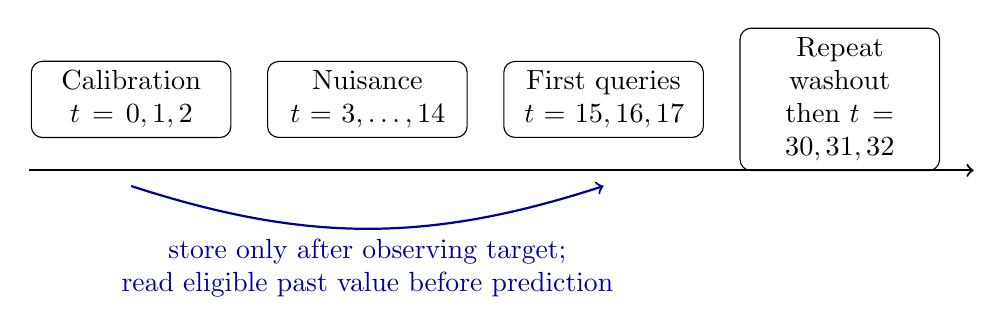
\begin{tikzpicture}[x=1cm,y=1cm]
\draw[->,thick] (0,0)--(12,0);
\node[draw,rounded corners,align=center,text width=2.3cm] at (1.3,0.9)
 {Calibration\\$t=0,1,2$};
\node[draw,rounded corners,align=center,text width=2.3cm] at (4.3,0.9)
 {Nuisance\\$t=3,\ldots,14$};
\node[draw,rounded corners,align=center,text width=2.3cm] at (7.3,0.9)
 {First queries\\$t=15,16,17$};
\node[draw,rounded corners,align=center,text width=2.3cm] at (10.3,0.9)
 {Repeat washout\\then $t=30,31,32$};
\draw[->,blue!60!black,thick] (1.3,-0.2) to[bend right=18]
 node[below,align=center]{store only after observing target;\\read eligible past value before prediction} (7.3,-0.2);
\end{tikzpicture}
\caption{One owner's event schedule. The paired owner receives the same query
context but the opposite residual. Each event predicts before its target is
written. Useful calibration-to-query age is 15 events in the first round.}
\label{fig:timeline}
\end{figure}

Owner identifiers are used as equality keys for bank routing, not as numerical
predictive features. The generator encodes regime in owner parity; any learner
allowed to exploit that encoding would have a different information set.
Anchor, regime, and query labels support generation, calibration selection,
and evaluation; ordinary retrieval does not use them to choose an entry.

\section{Executed residual-memory algorithm}
The frozen base is the last $c$ context channels, $B(X)=A$. After an event's
target is observed, its detached full context $K=X$ and residual $V=Y-B(X)$
are stored with owner, time, and an audit-only anchor label. Storage is FIFO
with capacity 128 per owner; the present streams contain only 33 entries each.
At each event time all predictions are completed before any target at that
time is written.

For ordinary retrieval, an entry is eligible if its owner equals the query
owner and $t-\tau_i\ge4$. Flattened keys and queries use cosine similarity,
with vector normalization floored at $10^{-8}$. The algorithm uses the top
one eligible item, and rejects it if similarity is below $0.999999$. Empty or
rejected retrieval yields zero correction. The implementation supports
softmax weighting with temperature $0.05$; with one item its weight is one.
The prediction is
\begin{equation}
 \widehat Y=B(X)+\alpha M(X,o,t),\qquad 0\le\alpha\le1.
\end{equation}
The stored key has $D_K=LcHW$ elements and the value $D_V=cHW$ elements.
Repeating an anchor $L$ times preserves cosine similarity, so full-context
and last-frame cosine comparisons are equivalent in this construction, but
the actual stored keys occupy $L$ times as many elements.

Let $J$ contain validation query rows with valid ordinary retrieval. The
closed-form calibration is
\begin{equation}
 \alpha=\Pi_{[0,1]}
 \frac{\sum_{j\in J}\langle Y_j-B_j,M_j\rangle}
      {\sum_{j\in J}\|M_j\|_2^2}.
\end{equation}
It is zero when the denominator is zero. Calibration is then fixed for all
test conditions; the oracle uses coefficient one. All retained seeds give
$\alpha=1$. No forecast model parameters are fitted.

The reference stores owners in one global list and filters that list on every
read. If there are $N$ total entries and $N_o$ entries for the queried owner,
retrieval costs $O(N+N_oD_K+D_V)$ for top one, with total tensor storage
$O(N(D_K+D_V))$. These are source-level complexity bounds, not measured
latency or an efficiency comparison. An indexed implementation could avoid the
global scan but is not the evaluated code.

\subsection{Conditions and their limitations}
All nine declared conditions are retained:
\begin{description}[style=nextline,leftmargin=1.0cm]
\item[Base / no memory] Compute retrieval but zero its correction. The bank is
still populated; this is an output ablation, not a memory-free timing baseline.
\item[Tensor memory] Use ordinary same-owner retrieval.
\item[Erase] Zero the retrieved value. In the executed code this has the same
prediction path as the base condition.
\item[Sign flip] Negate the retrieved value.
\item[Spatial mean] Average the value over spatial coordinates and broadcast
it. This deliberately removes a zero-mean innovation.
\item[Recent restriction] Apply maximum age 3 while retaining minimum age 4.
The eligibility set is empty. It is an empty-bank control, not evidence against
a functioning finite-history, recurrent, or recent-memory method.
\item[Last residual] Use the most recent age-eligible same-owner residual
without key matching. Nuisance residuals make it uninformative here.
\item[Paired swap] Route the query to the paired regime's bank, retaining the
past-time constraint. This deliberately relaxes ordinary owner isolation and
uses regime matching only as an oracle diagnostic.
\item[Oracle anchor] Select the most recent age-eligible same-owner entry with
the known anchor label. This label is unavailable to ordinary retrieval.
\end{description}
Swap success is defined by the executed predicate
\begin{equation}
 D_j=\mathbf1\!\left[\|\widehat Y_j^{\rm swap}-Y_j^{\rm donor}\|_2^2
       <\|B_j-Y_j^{\rm donor}\|_2^2\right].
\end{equation}
It compares distance to the donor against the base's distance to that donor;
it does not compare donor and recipient distances to the same prediction.

\section{Analytic expectations and diagnostic value}
\begin{proposition}[Context-only squared-error bound]
Fix an anchor $A$ and residual $R$ with paired targets $A\pm R$ of equal
weight. For any prediction $h(X)$ that is identical on the paired contexts,
its average per-element squared error is
$\|h(X)-A\|_2^2/(cHW)+\|R\|_2^2/(cHW)$, minimized by $h(X)=A$.
\end{proposition}
\begin{proof}
Expand the two squared norms for $A+R$ and $A-R$; their cross terms cancel.
The bound concerns an identical context-only output, not a predictor with
additional owner-derived information or an unrestricted recurrent state.
\end{proof}

In exact arithmetic, the base query MSE is $0.75^2=0.5625$. If a valid
matching entry supplies $rR$ and $\alpha=1$, prediction error is zero. Erasure
restores $rR$ error; sign reversal produces $2rR$ error and four times the
base MSE. Spatial averaging yields zero because $R$ is spatially centered.
Swapping to the paired residual $-rR$ equals the donor target and yields
$D_j=1$. The empty recent restriction yields the base prediction. These
identities explain the reported scores; they do not establish generalization.
Floating-point normalization accounts for small differences in stored MSE.

The same reasoning distinguishes three \emph{analytic counterexamples}, not
additional experimental runs. A program that reads the correct item but
always returns $A$ can have perfect retrieval precision yet fails the accuracy
gate. A program that obtains $rR$ through an oracle shortcut while ignoring
the memory value can have zero error yet fail erasure: deleting the memory
would change nothing. A correct exact dictionary lookup passes these
contrasts, just as the tested mechanism does. The diagnostic identifies an
information path under stated interventions; it cannot establish that ITFM is
architecturally better than an equivalent dictionary or another memory model.

\section{Protocol and retained results}
The development protocol records seeds 101, 211, and 307, fixed generation
parameters, all nine conditions, and decision thresholds. The retained
manifest binds that protocol and the executed source. This is a locally
specified development design; no external preregistration is asserted.
The protocol hash and unchanged outcome records are retained for inspection.
The stopping rule is the fixed set of three seeds and nine conditions; this
revision adds no tuning, exclusions, or replacement seeds.

For any subset $S$, the executed estimator pools squared errors:
\begin{equation}
 \mathrm{NMSE}(S)=
 \frac{\sum_{j\in S}\|Y_j-\widehat Y_j\|_2^2}
      {\sum_{j\in S}cHW}\frac{1}{\sigma^2_{\rm train}},
\end{equation}
where $\sigma^2_{\rm train}$ is the population variance of all flattened
training targets, computed with no degrees-of-freedom correction. Each owner
has six query and 27 non-query rows of equal size; each family has two owners.
Consequently pooling equals owner-then-family averaging for each subset in
this balanced corpus. This equivalence need not hold for unequal streams.

Dataset validation checks disjoint/exhaustive family splits and paired
contexts, futures, and ages. Five recorded identifiability predicates cover
full-context equality, nonzero future difference, age beyond context,
last-two-frame equality, and at least 20\% validation oracle gain. The last
predicate is measured on validation; test labels are not used to calibrate
$\alpha$. Generator integrity is checked on all splits, so the synthetic test
is not an externally blinded confirmatory dataset.

The eight numerical predicates require: at least 5\% query improvement over
each of base, sign flip, spatial mean, recent restriction, and last residual;
at least 50\% oracle-gap recovery; at least 80\% gain removal under erasure;
swap success at least 0.90; retrieval precision at least 0.99; non-query NMSE
increase at most 0.01; sign-flip error strictly above ordinary retrieval; and
spatial-mean error strictly above ordinary retrieval. Source/artifact integrity
is checked separately. A failing seed or condition cannot be discarded to
produce a pass.

% Generated from unchanged retained records by publication tools/release.py.
\begin{table}[ht]\centering\small
\caption{Query NMSE for every declared condition and seed. Each cell uses 108 query rows. Paired-swap error is measured against the recipient target, while its diagnostic success rate below concerns the donor.}
\label{tab:results}\begin{tabular}{lrrr}\toprule
Condition & 101 & 211 & 307 \\\midrule
Base output & 0.487685 & 0.487685 & 0.487685 \\
Tensor memory & 0.000000 & 0.000000 & 0.000000 \\
Erase & 0.487685 & 0.487685 & 0.487685 \\
Sign flip & 1.950739 & 1.950739 & 1.950739 \\
Spatial mean & 0.487685 & 0.487685 & 0.487685 \\
Recent restriction (empty) & 0.487685 & 0.487685 & 0.487685 \\
Last residual & 0.487685 & 0.487685 & 0.487685 \\
Paired swap & 1.950739 & 1.950739 & 1.950739 \\
Oracle anchor & 0.000000 & 0.000000 & 0.000000 \\
\bottomrule\end{tabular}\end{table}
\begin{table}[ht]\centering\small
\caption{Additional retained diagnostics. Non-query metrics use 486 rows per seed. Precision and donor success use the relevant valid query retrievals.}
\begin{tabular}{lrrr}\toprule
Metric & 101 & 211 & 307 \\\midrule
Base non-query NMSE & 0.054187 & 0.054187 & 0.054187 \\
Tensor non-query NMSE & 0.054187 & 0.054187 & 0.054187 \\
Matching-anchor precision & 1.000000 & 1.000000 & 1.000000 \\
Donor improvement rate & 1.000000 & 1.000000 & 1.000000 \\
\bottomrule\end{tabular}\end{table}

The three retained seeds pass the eight numerical predicates. The test
normalization gives base query NMSE near $0.487685$. Ordinary retrieval and
the oracle have zero query error. Non-query NMSE is approximately $0.0541872$
for both ordinary retrieval and the base. All query retrievals in the ordinary
condition match their anchor, and all valid paired-swap queries satisfy $D_j$.
Three seeds measure repeatability of this fixed construction. We report their
values directly rather than infer a natural-domain population effect or
present the near-identical numbers as a powered estimate of robustness.

\section{Verification and reproducibility boundary}
The original manifest reports Python 3.11.15 and Torch 2.12.1. Its 20-file
executed source bundle has been recovered and verified byte-for-byte, including
the original project metadata that had been replaced by later public-stack
packaging. Original results and failed receipts are retained unchanged. The
historical full dependency lock was not recorded; source recovery alone does
not reconstruct every environmental dependency.

The historical local verifier passed 96 checks. The files named
\texttt{predictions-*.json} contain scalar squared errors, element counts,
retrieval metadata, and donor-success booleans, not raw prediction and target
tensors. Thus the original verifier reaggregates these records and checks
hashes and decision consistency. It reads saved data-identifiability flags;
it does not independently regenerate that evidence. A current check against
the recovered source can verify historical source identity without claiming
a new execution of the model. Raw-output replay and external reproduction
are separate requirements and are not represented by that historical pass.

A non-overwriting reproduction wrapper accompanies the revision. It uses an
isolated copy of the executed source and fresh outputs, rather than calling
the historical runner against the archived result directory. New verification
receipts must state their source, environment, comparison tolerances, and
whether they concern records, tensors, or independent execution. No external
reproduction or public-data experiment is claimed here.

From the companion archive's synthetic-study root, the lightweight check is
\texttt{python3 scripts/build\_paper\_release.py verify}. For replay, first
enter \texttt{publication/itfm-v2-paper-20261011}, then run
\texttt{python3 tools/reproduce.py execute --output replays/NEW}.
The output path must not exist. The wrapper checks the fixed resource floor
before importing Torch and imposes a 300-second limit per step with one
numerical thread. A blocked admission is retained and is not a failed
scientific outcome. The wrapper's local environment is not an independent
reproduction or a substitute for a resolved, clean dependency installation.

\section{Limitations and future work}
The system is a deliberately easy exact-lookup construction with repeated
keys, stationary residuals, one grid size, and unused capacity headroom. It
cannot support claims about learned keys, noise, drift, changing grids,
continuous trajectories, imperfect owner identity, public PDEs, or deployment.
The recent restriction is empty and the base/erase paths coincide; these
controls must not be presented as independent strong baselines. Later query
rounds may retrieve an earlier query's residual as well as calibration entries.
Equal-score ordering is inherited from Torch top-$k$; equal repeated-anchor
values make those ties prediction-equivalent here, not in arbitrary tasks.

The interventions localize a path in a fixed program. They do not prove that
all other implementation dependencies are excluded or identify a causal effect
in observational physics. A useful next evaluation would freeze meaningful
recent-history and trained sequence controls, approximate/noisy keys, and
natural partial-observation tasks before outcome access. The prospective
ITFM-R public campaign is deferred and supplies no claim in this paper.

\section{Data availability and disclosures}
The study uses generated fields and no human-subject data. Owner identifiers
are synthetic routing labels. The local companion materials contain the
protocol, exact recovered source, original records, claim map, and verification
instructions. A publicly retrievable immutable archive and its distribution
terms have not yet been finalized; no public download availability is claimed.
Authorship is single-author. AI assistance was used for
code/manuscript revision and evidence auditing; it does not constitute an
independent scientific reviewer or reproducer. No measured energy-efficiency
or public benchmark performance claim is made.

\section{Conclusion}
Under the declared exact alias construction, a past spatial residual provides
information absent from the identical visible context. The reference lookup
reuses it, and erasure, sign reversal, pooling, and diagnostic owner swaps have
the predicted effects. This bounded result is an inspectable mechanism case
study. Its exact score and local record checks do not establish a new learning
architecture, robust forecasting benefit, or independent reproduction.

\bibliographystyle{plain}
\bibliography{references}
\end{document}
